In this section, we present an approach to uncertainty quantification that forms
the core of the proposed framework. The approach belongs to the class of
stochastic collocation techniques \cite{xiu2010}. The major distinctive feature
of stochastic collocation is the usage of interpolation as a means of
uncertainty quantification, which should be contrasted with other techniques
such as polynomial chaos expansions relying on regression. The interpolation
algorithm that we use was developed in \cite{klimke2006} and \cite{ma2009}, and
it features a sparse-grid structure, hierarchical construction, and local
adaptivity. The sparse-grid structure is to address the curse of dimensionality
and, hence, tackle high-dimensional problems; the hierarchical construction is
to have a gradual refinement of approximation with a natural error control;
and the local adaptivity is to make the refinement fine-grained and, hence, gain
further efficiency.

Let $\f$ be an uncertain quantity that we are interested in studying. The
quantity is viewed as a vector of $\nout$ deterministic functions each of which
is parametrized by the same set of $\nin$ random variables. Each function
belongs to $\continuous([0, 1]^\nin)$, the space of continuous functions defined
on the unit hypercube $[0, 1]^\nin$. Thus, we have
\[
  \f: [0, 1]^\nin \to \real^\nout \subset \continuous([0, 1]^\nin).
\]
Note that the domain $[0, 1]^\nin$ is not a restriction.

The function is assumed to be computationally intensive and impractical for
extensive evaluation, which is needed for Monte Carlo sampling. For example, the
concise notation $\f$ might expand into a full-system simulation, including
scheduling and power-temperature analysis, which is the case in this work.

In order to make the problem computationally tractable, a light representation
of $\f$ is constructed and studied instead of $\f$. The surrogate is based on
interpolation: $\f$ is evaluated at a small number of points or nodes, and any
other values of $\f$ are reconstructed on demand using a set of basis functions
mediating between the obtained values of $\f$.

In what follows, we shall gradually construct an efficient interpolant for $\f$.
\emph{Efficiency}, in this context, refers to the number of nodes required to
achieve a certain accuracy level.

\subsection{Tensor Product} \slab{tensor-product}
In one dimension ($\nin = 1$), $\f$ is approximated by virtue of the following
interpolation formula:
\begin{equation} \elab{tensor-1d}
  \tensor{i}(\f) = \sum_{j \in \oindex_i} \f(\x_{ij}) \, \e_{ij}
\end{equation}
where $i \geq 0$ signifies the level of interpolation; $\X_i = \{ \x_{ij} \}_{j
\in \oindex_i} \subset [0, 1]$ are the collocation nodes; $\E_i = \{ \e_{ij}
\}_{j \in \oindex_i} \subset \continuous([0, 1])$ are the basis functions; and
$\oindex_i = \{ j - 1 \}_{j = 1}^{n_i}$ is an index set enumerating (starting
from zero) the nodes and functions of level $i$. The subscript $j \in \oindex_i$
is referred to as the order of a node or function. The choice of $\X_i$ and
$\E_i$ is important and will be discussed thoroughly later on.

In multiple dimensions ($\nin > 1$), $\f$ is approximated by the tensor product
of $\nin$ one-dimensional interpolants:
\begin{equation} \elab{tensor}
  \tensor{\vi}(\f) = \left( \bigotimes_{k = 1}^\nin \tensor{i_k} \right)(\f) = \sum_{\vj \in \oindex_\vi} \f(\vx_{\vi\vj}) \, \e_{\vi\vj}
\end{equation}
where $\vi = (i_k)_{k = 1}^\nin$ and $\vj = (j_k)_{k = 1}^\nin$ are
multi-indices specifying levels and orders, respectively, for each of the
dimensions, and $\oindex_\vi = \oindex_{i_1} \times \cdots \times
\oindex_{i_\nin}$ is a multi-index set obtained by computing the tensor product
of one-dimensional index sets. In the above formula,
\begin{align}
  \X_\vi &= \X_{i_1} \times \cdots \times \X_{i_\nin} \elab{collocation-nodes} \\
         &= \left\{ \vx_{\vi\vj} = (\x_{i_k j_k})_{k = 1}^\nin \right\}_{\vj \in \oindex_\vi} \subset [0, 1]^\nin \nonumber
\end{align}
and
\begin{equation} \elab{basis-functions}
  \E_\vi = \bigotimes_{k = 1}^\nin \E_{i_k}
         = \left\{ \e_{\vi\vj} = \bigotimes_{k = 1}^\nin \e_{i_k j_k} \right\}_{\vj \in \oindex_\vi} \subset \continuous([0, 1]^\nin)
\end{equation}
are the collocation nodes and basis functions, respectively, corresponding to
multi-index $\vi$. In \eref{basis-functions}, for any $\vx \in [0, 1]^\nin$,
\begin{equation} \elab{basis-function}
  \e_{\vi\vj}(\vx) = \left( \bigotimes_{k = 1}^\nin \e_{i_k j_k} \right)(\vx) = \prod_{k = 1}^\nin \e_{i_k j_k}(\x_k).
\end{equation}
Lastly, the cardinality of $\oindex_\vi$ is as follows:
\begin{equation} \elab{tensor-cardinality}
  \n_\vi = \prod_{k = 1}^\nin \n_{i_k}.
\end{equation}
Equation \eref{tensor-cardinality} elucidates the prohibited expense of the
tensor-product construction shown in \eref{tensor} for multidimensional
problems: the number of nodes grows exponentially as $\nin$ increases. However,
\eref{tensor} serves well as a building block for more efficient algorithms,
which we discuss next.

\begin{remark}
Each dimension can have its own rule defining the distribution of collocation
node with respect to each level. Similarly, the basis functions of one dimension
can differ from the basis functions of another. For simplicity and clarity of
presentation, this aspect is not covered in this paper.
\end{remark}


\subsection{Smolyak Algorithm} \slab{smolyak-algorithm}
One of the central algorithms in the field of multidimensional integration and
interpolation is the Smolyak algorithm \cite{smolyak1963}. The technique was
developed in the 1960s by Sergey Smolyak, and its impact is comparable to the
one of Monte Carlo sampling. Intuitively speaking, the algorithm takes a number
of small tensor-product structures and composes them in such a way that the
resulting grid has a drastically reduced number of nodes while preserving the
approximating power of the full tensor-product construction for the classes of
functions that one is typically interested in integrating or interpolating
\cite{klimke2006}.

The Smolyak interpolant for $\f$ is as follows:
\begin{equation} \elab{smolyak-original}
  \smolyak{\l}(\f) = \sum_{\l - \nin + 1 \leq |\vi| \leq \l} (-1)^{\l - |\vi|} \, {\nin - 1 \choose \l - |\vi|} \, \tensor{\vi}(\f)
\end{equation}
where $\l \geq 0$ is the level of Smolyak's interpolation, and $|\vi| = i_1 +
\dots + i_\nin$. We see that the algorithm is indeed just a peculiar composition
of cherry-picked tensor products. However, the formula has an implication of
paramount importance. The quantity of interest needs to be evaluated only at the
nodes of the sparse grid underpinning \eref{smolyak-original}:
\begin{equation} \elab{smolyak-grid}
  \Y_l = \bigcup_{\l - \nin + 1 \leq |\vi| \leq \l} \X_\vi.
\end{equation}
The cardinality of the above set does not have a general closed-form formula;
however, it can be several orders of magnitude smaller than the one of the full
tensor product given in \eref{tensor-cardinality}, which depends on the
dimensionality of the problem at hand and the one-dimensional rules utilized.

A better intuition about the properties of Smolyak's construction can be
obtained by rewriting \eref{smolyak-original} in an incremental form. To this
end, let $\Delta\tensor{-1}(\f) = 0$,
\begin{align}
  & \Delta\tensor{i}(\f) = (\tensor{i} - \tensor{i - 1})(\f), \text{ and} \elab{tensor-delta-1d} \\
  & \Delta\tensor{\vi}(\f) = \left( \bigotimes_{k = 1}^\nin \Delta\tensor{i_k} \right)(\f). \nonumber
\end{align}
Then, \eref{smolyak-original} is identical to
\begin{equation} \elab{smolyak-incremental}
  \smolyak{\l}(\f) = \sum_{\vi \in \lindex_\l} \Delta\tensor{\vi}(\f) = \smolyak{\l - 1}(\f) + \sum_{\vi \in \Delta\lindex_\l} \Delta\tensor{\vi}(\f)
\end{equation}
where $\smolyak{-1}(\f) = 0$, and we let $\lindex_\l = \{ \vi: |\vi| \leq \l
\}$ and $\Delta\lindex_\l = \{ \vi: |\vi| = \l \}$. It can be seen that a
Smolyak interpolant can be refined efficiently: the work done in order to attain
one accuracy level is entirely recycled to go to the next.

The sparsity and incremental refinement of Smolyak's approach, which are shown
in \eref{smolyak-grid} and \eref{smolyak-incremental}, respectively, are
remarkable properties \perse, but they can be taken even further. To this end,
let $\Delta\X_{-1} = \emptyset$,
\begin{align*}
  & \Delta\X_i = \X_i \setminus \X_{i - 1}, \text{ and} \\
  & \Delta\X_\vi = \Delta\X_{i_1} \times \cdots \times \Delta\X_{i_\nin}.
\end{align*}
Then, \eref{smolyak-grid} can be rewritten as
\begin{equation} \elab{smolyak-grid-incremental}
  \Y_\l = \bigcup_{\vi \in \lindex_\l} \Delta\X_\vi = \Y_{\l - 1} \cup \bigcup_{\vi \in \Delta\lindex_\l} \Delta\X_\vi,
\end{equation}
which is analogous to \eref{smolyak-incremental}. It can be seen now that it is
beneficial for refinement to have $\X_{i - 1}$ be entirely included in $\X_i$
since, in that case, the cardinality of $\Y_l \setminus \Y_{\l - 1} =
\bigcup_{\vi \in \Delta\lindex_\l} \Delta\X_\vi$ derived from
\eref{smolyak-grid-incremental} decreases. In words, the values of $\f$ obtained
on lower levels can be reused to attain higher levels if the grid grows without
abandoning its previous structure. With this in mind, the rule used for
generating successive sets of points $\{ \X_i \}_i$ should be chosen to be
nested, that is, in such a way that $\X_i$ contains all nodes of $\X_{i - 1}$.
By doing so, the incremental refinement really starts to shine.

The final step in this subsection is to rewrite \eref{smolyak-incremental} in a
hierarchical form. To this end, we require the interpolants of higher levels to
represent exactly the interpolants of lower levels. In one dimension, it means
that
\begin{equation} \elab{tensor-exactness}
  \tensor{i - 1}(\f) = \tensor{i}(\tensor{i - 1}(\f)).
\end{equation}
The condition in \eref{tensor-exactness} can be satisfied by an appropriate
choice of collocation nodes and basis functions, which will be discussed later.
If \eref{tensor-exactness} holds, using \eref{tensor-1d} and
\eref{tensor-delta-1d},
\[
  \Delta\tensor{i}(\f) = \sum_{j \in \Delta\oindex_i} \left( \f(\x_{ij}) - \tensor{i - 1}(\f)(\x_{ij}) \right) \, \e_{ij}
\]
where $\Delta\oindex_i = \{ j \in \oindex_i: \x_{ij} \in \Delta\X_i \}$. The
above sum is over $\Delta\X_i$ due to the fact that the difference in the
parentheses is zero whenever $\x_{ij} \in \X_{i - 1}$ since $\X_{i - 1} \subset
\X_i$.

In multiple dimensions, using the Smolyak formula,
\begin{equation} \elab{tensor-delta}
  \Delta\tensor{\vi}(\f) = \sum_{\vj \in \Delta\oindex_\vi} \left( \f(\vx_{\vi\vj}) - \smolyak{|\vi| - 1}(\f)(\vx_{\vi\vj}) \right) \, \e_{\vi\vj}
\end{equation}
where $\Delta\oindex_\vi = \{ \vj \in \oindex_\vi: \vx_{\vi\vj} \in
\Delta\X_\vi \}$. The delta
\begin{equation} \elab{surplus}
  \surplus(\vx_{\vi\vj}) = \f(\vx_{\vi\vj}) - \smolyak{|\vi| - 1}(\f)(\vx_{\vi\vj})
\end{equation}
is called a hierarchical surplus. When increasing the interpolation level, this
surplus is nothing but the difference between the actual value of $\f$ at a new
node and the approximation of this value computed by the interpolant constructed
so far.

The final formula for nonadaptive hierarchical interpolation is obtained by
substituting \eref{tensor-delta} into \eref{smolyak-incremental}:
\begin{align}
  \smolyak{\l}(\f) &= \sum_{\vi \in \lindex_\l} \, \sum_{\vj \in \Delta\oindex_\vi} \surplus(\vx_{\vi\vj}) \, \e_{\vi\vj} \elab{smolyak-hierarchical} \\
                   &= \smolyak{\l-1}(\f) + \sum_{\vi \in \Delta\lindex_\l} \, \sum_{\vj \in \Delta\oindex_\vi} \surplus(\vx_{\vi\vj}) \, \e_{\vi\vj} \nonumber
\end{align}
where $\surplus(\vx_{\vi\vj})$ is computed according to \eref{surplus}.


\subsection{Adaptivity}
Imagine a function that is nearly flat on the first half of $[0, 1]$ and rather
irregular on the other. Under these circumstances, it is natural to expect that,
in order to attain the same accuracy, the first half would require much fewer
collocation nodes than the other one; recall \fref{motivation}. However, if we
followed the construction procedure described so far, we would not be able to
benefit from the peculiar behavior: we would treat both sides equally and would
add all the nodes of each level.

The solution to the above problem is to make the interpolation algorithm
adaptive. To this end, we first need to find a way to measure how good our
approximation is at any point in the domain of $\f$. Then, when refining the
interpolant, instead of bombarding $\f$ with all possible nodes, we will only
choose those that are located in the regions with poor accuracy as indicated by
the yet-to-be-found accuracy metric.

Thanks to the hierarchical form obtained in the previous subsection, we already
have a good material for building an accuracy metric. Recall \eref{surplus}.
Hierarchical surpluses are natural indicators of the interpolation error: they
are the difference between the true function and its approximation at the nodes
of the underlying sparse grid. Hence, they can be recycled in order to
effectively identify ``problematic'' regions. Specifically, we first assign a
score to each node $\vx_{\vi\vj}$ or, equivalently, to each pair of level and
order indices $(\vi, \vj)$:
\begin{equation} \elab{score}
  \score_{\vi\vj} = \left| \surplus(\vx_{\vi\vj}) \, \w_{\vi\vj} \right|
\end{equation}
where $\surplus(\vx_{\vi\vj})$ and $\w_{\vi\vj}$ are given by \eref{surplus} and
\eref{volume}, respectively, and this score is then used in order to guide the
algorithm as we shall explain in the rest of this subsection.

The Smolyak construction in \eref{smolyak-hierarchical} is rewritten as follows:
\begin{equation} \elab{approximation}
  \approximation{\l}(\f) = \approximation{\l-1}(\f) + \sum_{\vi \in \Delta\lindex_\l} \sum_{\vj \in \Delta\oindex_\vi} \surplus(\vx_{\vi\vj}) \,
\e_{\vi\vj}.
\end{equation}
The main different with respect to \eref{smolyak-hierarchical} is that $\l \geq
0$ no longer signifies a Smolyak level but a more abstract interpolation step,
and $\approximation{\l}$ is the interpolant at that step. As always,
$\approximation{-1} = 0$, and the definition of $\surplus$ given in
\eref{surplus} is adjusted accordingly. Lastly, all index sets from now on are
generally subsets of their full-fledged counterparts defined in
\sref{smolyak-algorithm}.

\begin{remark}
All the rules below make sure that the construction in \eref{approximation}
adhere to the same principles as the ones underpinning
\eref{smolyak-hierarchical}. An arbitrary construction is generally invalid.
\end{remark}

Each $\approximation{\l}$ is characterized by a set of level indices
$\lindex_\l$, and each $\vi \in \lindex_\l$ by a set of order indices
$\Delta\oindex_\vi$. At each interpolation step $\l \geq 0$, a single index
$\vi_\l$ is chosen from $\lindex_{\l-1}$ with $\lindex_{-1} = \{ \v{0} \}$. The
chosen index then gives birth to $\Delta\lindex_\l$ and $\{ \Delta\oindex_\vi
\}_{\vi \in \Delta\lindex_\l}$, which shape the increment in the right-hand side
of \eref{approximation}.

The set $\Delta\lindex_\l$ contains the so-called admissible forward neighbors
of $\vi_\l$. Let us now parse the previous sentence. First, the forward
neighbors of an index $\vi$ are given by
\begin{equation} \elab{forward-level-neighbors}
  \left\{ \vi + \v{1}_k: k = 1, \dots, \nin \right\}
\end{equation}
where $\v{1}_k$ is a vector whose elements are zero except for element $k$ equal
to unity. Next, an index $\vi$ is admissible if its inclusion into the index set
in question $\lindex$ keeps the set admissible. Finally, $\lindex$ is admissible
if it satisfies the following condition \cite{klimke2006}:
\begin{equation} \elab{admissibility}
  \vi - \v{1}_k \in \lindex, \text{ for $\vi \in \lindex$ and $k = 1, \dots, \nin$,}
\end{equation}
where, naturally, the cases with $i_k = 0$ need no check.

Now, how is $\vi_\l$ chosen from $\lindex_{\l-1}$ at each iteration of
\eref{approximation}? First of all, each index can be obviously picked at most
once. The rest is resolved by prioritizing the candidates. It is reasonable to
assign a priority to a level index $\vi$ based on the scores of the order
indices associated with it, that is, on the scores of $\oindex_\vi$. We compute
the priority as the average score:
\[
  \score_\vi = \frac{1}{\card{\Delta\oindex_\vi}} \sum_{\vj \in \Delta\oindex_\vi} \score_{\vi\vj}
\]
Consequently, the answer to the above question is that, at each step $\l$, the
index $\vi$ with the highest $\score_\vi$ gets promoted to $\vi_\l$.

Let us now turn to the content of $\Delta\oindex_\vi$ where $\vi = \vi_\l +
\v{1}_k$ for a fixed $k$. It also contains admissible forward neighbors, but
they are order indices, and their construction is drastically different from the
one in \eref{forward-level-neighbors}. Concretely, these indices are identified
by inspecting the backward neighborhood of $\vi$ (analogous to
\eref{forward-level-neighbors}). For each backward neighbor $\hat{\vi} = \vi -
\v{1}_{\hat{k}}$ and each $\vj \in \Delta\oindex_{\hat{\vi}}$, we begin by
checking the following condition:
\[
  \score_{\hat{\vi}\vj} \geq \serror
\]
where $\serror$ is a user-defined constant referred to as the score error. If
the condition holds, the forward neighbors of $\vj$ in dimension $k$ are added
to $\Delta\oindex_\vi$. This procedure for the open Newton--Cotes rule is
illustrated in \fref{rule}. The arrows emerging from a node connect the node
with its forward neighbors. It can be seen that each node has two forward
neighbors (for one dimension); their order indices are
\[
  (j_1, \dots, 2 j_k, \dots, j_\nin) \hspace{1em} \text{and} \hspace{1em} (j_1, \dots, 2 j_k + 2, \dots, j_\nin).
\]
The above refinement procedure is repeated for each index $\vi \in
\Delta\lindex_\l$ with respect to each dimension $k = 1, \dots, \nin$.

The final question is the stopping condition of the approximation process in
\eref{approximation}. Apart from the obvious constraints on the maximum number
of function evaluations and deepness of interpolation (the Smolyak level), we
rely on the following criterion. Assume given two additional constants:
$\aerror$ and $\rerror$ referred to as the absolute and relative error,
respective. Then, the process is terminated as soon as
\[
  \max_{(\vi, \vj)} \, |\surplus(\vx_{\vi\vj})| \leq \max \left\{ \aerror, \, \rerror (\f_\text{max} - \f_\text{min}) \right\}
\]
where $\f_\text{min}$ and $\f_\text{max}$ the minimum and maximum observed
values of $\f$, respectively, and the left-hand side is the maximum surplus
whose level index has not been refined yet (considered as $\vi_\l$ at some step
$\l$ in \eref{approximation}). The above criterion is a sound way to curtail the
process it is based on the actual progress.

The adaptivity presented in this subsection is referred to as hybrid as it
exhibits features of both global and local adaptivity. Local adaptivity operates
on the level of individual nodes, and it has already been motivated. Global
adaptivity operates on the level of individual dimensions. The intuition behind
it is that, in general, the input variables manifest themselves (impact $\f$)
differently, and the interpolation algorithm is likely to benefit by
prioritizing those variables that the most influential.


\subsection{Collocation Nodes} \slab{collocation-nodes}
A sparse grid that is fully nested and well suited for local adaptivity, which
we required previous, can be constructed using the (one-dimensional)
Newton--Cotes rule \cite{klimke2006, ma2009}. For each level, the rule is merely
a set of equidistant nodes on an interval, which is $[0, 1]$ in our case.

\begin{remark}
Equidistant nodes are known to perform purely when the interpolating functions
are chosen to be polynomials (Runge's phenomenon). However, it is not a concern
for us as our basis functions are not exposed to this problem.
\end{remark}

The rule comes in two flavors: closed and open. The only difference between the
two is that the former includes the endpoints, that is, 0 and 1, while the
latter does not. Now, at the end of \sref{smolyak-algorithm}, we postulated that
the assumption in \eref{tensor-exactness} was needed to proceed. The closed rule
satisfies this assumption while the open one violates it close to the boundaries
of the interval. However, according to our numerical experiments and as noted in
\cite{klimke2006}, the open Newton--Cotes rule is a viable option as it performs
well in practice.

Despite the minor concern noted above, we have opted to present the open
Newton--Cotes rule in the paper as it is a better match for the transformation
in \eref{transformation}. The problem with 0 and 1 is rather technical and is as
follows. The inverse of the Gaussian distribution function, $\Phi^{-1}$, maps 0
and 1 to $-\infty$ and $+\infty$, respectively; as shown in
\eref{transformation}, the resulting vector then gets multiplied by a matrix.
Now, since certain algebraic operations with infinite values are undefined---for
instance, $0.42 \times (+\infty) + 0.27 \times (-\infty)$---this particular
transformation in \eref{transformation} might pose implementation difficulties,
which we would like to avoid by choosing a rule without the endpoints.

\begin{figure}[t]
  \centering
  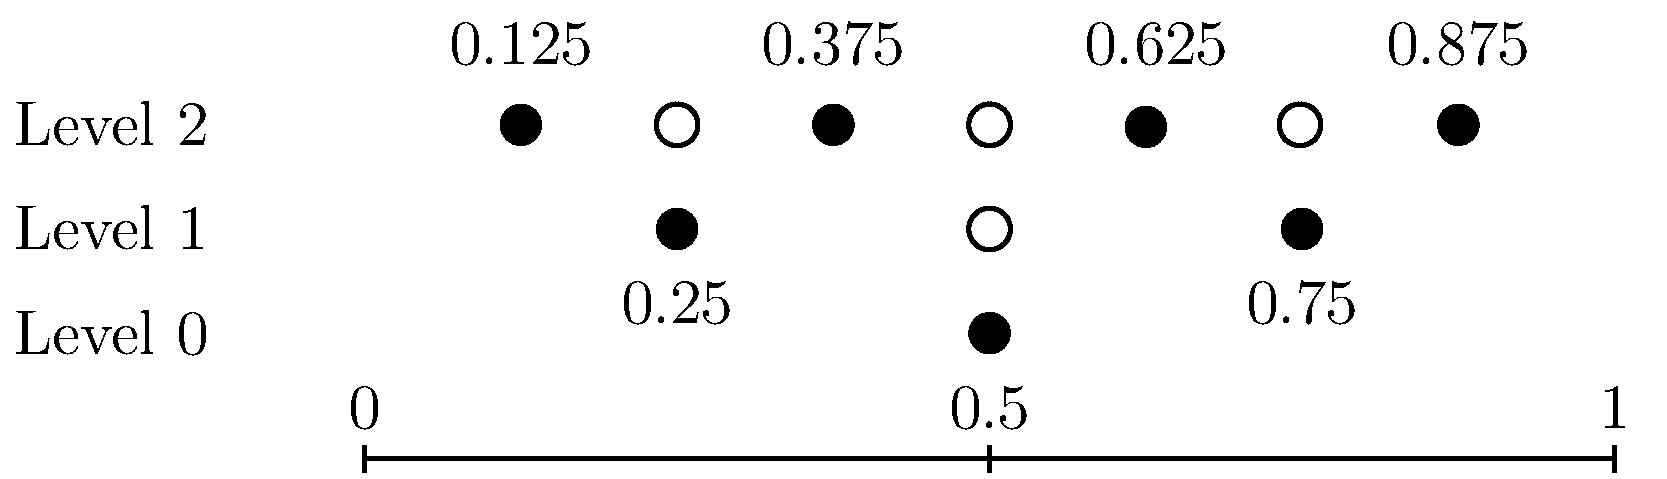
\includegraphics[width=1.0\columnwidth]{include/assets/rule.pdf}
  \caption{
    An illustration of the open Newton--Cotes rule on $[0, 1]$. On each level,
    the dots correspond to the nodes introduced by that particular level, and
    the wholes correspond to the nodes inherited from the previous levels.
  }
  \flab{rule}
\end{figure}

The open Newton--Cotes rule of level $i \in \natural$ is
\[
  \X^i = \left\{ x^i_j = \frac{j + 1}{\n_i + 1}: j \in \index(i) \right\}
\]
where $\index(i) = \left\{ 0, \dots, \n_i - 1 \right\}$ with $\n_i = 2^{i + 1} -
1$. The first three levels of the rule are depicted in \fref{rule}. It can be
seen that the number of nodes (in one dimension) grows as 1, 3, 7, 15, 31, and
so on, and the rule is fully nested. In multiple dimensions, the nodes are
formed as shown in \eref{collocation-nodes}.

\fref{rule} also illustrates the refinement strategies suitable for this grid.
The arrows emerging from a node connect the node with its next-level neighbors.
The number of such neighbors is two in one dimension and $2 \nin$ in general.
Formally, for a pair $(\vi, \vj)$, the neighbor pairs are
\[
  \left\{ \Big( (i_1, \dots, i_k + 1, \dots, i_\nin), (j_1, \dots, 2 j_k + c, \dots j_\nin) \Big) \right\}_{k, c}
\]
for $k = 1, \dots, \nin$ and $c \in \{ 0, 2 \}$. Whenever a node is to be
refined, some or all of its neighbors can be chosen for function evaluation. The
simplest strategy is to include all $2 \nin$ neighbors, which is what we shall
do.


\subsection{Basis Functions} \slab{basis-functions}
\begin{figure}[t]
  \centering
  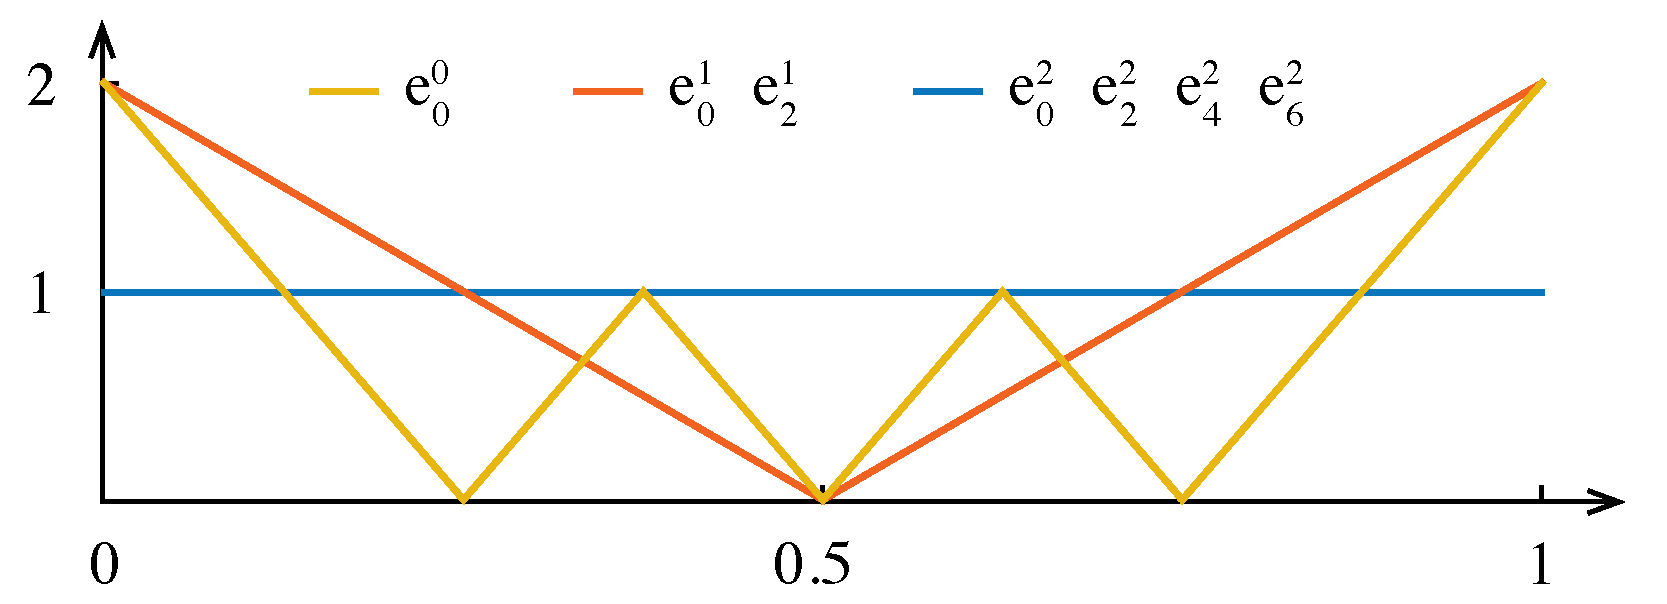
\includegraphics[width=1.0\columnwidth]{include/assets/figures/basis.pdf}
  \vspace{-1.5em}
  \caption{
    The first three levels of the basis described in \sref{basis}.
  }
  \flab{basis}
\end{figure}

The basis functions that go hand in hand with the open Newton--Cotes rule are
the following piecewise linear functions. For $i = 0$ and $j = 0$,
\[
  \e_{00}(\x) = 1.
\]
For $i > 0$ and $j = 0$ (close to the left endpoint),
\[
  \e_{i0}(\x) = \begin{cases}
    2 - \left( \n_i + 1 \right) \x, & \text{if } \x < \frac{2}{\n_i + 1}, \\
    0, & \text{otherwise}.
  \end{cases}
\]
For $i > 0$ and $j = \n_i - 1$ (close to the right endpoint),
\[
  \e_{i(\n_i - 1)}(\x) = \begin{cases}
    \left( \n_i + 1 \right) \x - \n_i + 1, & \text{if } \x > \frac{\n_i - 1}{\n_i + 1}, \\
    0, & \text{otherwise}.
  \end{cases}
\]
In other cases,
\[
  \e_{ij}(\x) = \begin{cases}
    1 - \left( \n_i + 1 \right)|\x - \x_{ij}|, & \text{if } |\x - \x_{ij}| < \frac{1}{\n_i + 1}, \\
    0, & \text{otherwise}.
  \end{cases}
\]
The basis functions corresponding to the first three levels of one-dimensional
interpolation are depicted in \fref{basis}. Note that $\e_{11}$, $\e_{21}$,
$\e_{23}$, and $\e_{25}$ are not depicted as they are not involved in the
hierarchical construction. In multiple dimensions, the basis functions are
formed as shown in \eref{basis-functions}.

Lastly, let us mention the volumes (integrals over the whole domain) of the
basis functions denoted by $\w_{ij}$; they will be needed in the future. Namely,
$\w_{00} = 1$ and, for $i > 0$,
\begin{equation} \elab{volume}
  \w_{ij} := \int_0^1 \e_{ij}(\x) \, \d\x = \begin{cases}
    \frac{2}{\n_i + 1}, & \text{if } j \in \{ 0, \n_i - 1 \}, \\
    \frac{1}{\n_i + 1}, & \text{otherwise}.
  \end{cases}
\end{equation}
In multiple dimensions, the volumes are products of the one-dimensional
components, analogous to \eref{basis-function}.

\begin{remark}
Instead of piecewise linear functions, one can also utilize locally supported
polynomials of higher orders \cite{jakeman2012}. However, we did not observe
much improvement and, therefore, do not discuss this alternative in the paper.
\end{remark}


\subsection{Implementation}
The life cycle of interpolation has roughly two stages: construction and usage.
The construction stage invokes $\f$ at a set of collocation nodes and produces
certain artifacts. The usage stage estimates the values of $\f$ at a set of
arbitrary points by manipulating the artifacts. In this subsection, we shall
look at the pseudocodes of the two stages. The purpose is to give the big
picture. A lot of implementation details are purposely omitted; however, all the
details can be found and studied online as our implementation is open source
\cite{sources}.

Let us first make a general note. We found it beneficial to the clarity and ease
of implementation to collapse the two sums in \eref{approximation} into one.
This requires storing a level index $\vi = (i_k)_{k = 1}^\nin$ and an order
index $\vj = (j_k)_{k = 1}^\nin$ for each interpolation element. It is also
advantageous to encode each pair $(i_k, j_k)$ as a single unsigned integer,
which, in particular, eliminates excessive memory usage. In multiple dimensions,
this results in a single vector $\vl = (\iota_k)_{k = 1}^\nin$, which we simply
call an index. The encoding that we utilize is as follows:
\[
  \iota_k = i_k \lor (j_k \ll \n_\text{bits})
\]
where $\lor$ and $\ll$ are the bitwise \up{OR} and logical left shift,
respectively, and $\n_\text{bits}$ is the number of bits reserved for storing
Smolyak levels, which can be adjusted according to the maximum permitted
deepness of interpolation.

The pseudocode of the construction stage is given in \aref{construct} called
\token{Construct}. The \token{target} input is a function $\f$ to be
approximated. The \token{surrogate} output is a structure containing the
artifacts of interpolation, which are a set of tuples $\{ (\vl_k,
\surplus(\vx_{\vl_k}) \}_k$, giving a comprehensive description of an
interpolant. The routine works as follows.

\begin{compactlist}

\point{Line~2:} Each iteration is an interpolation step in \eref{approximation}.
It has a state captured by a structure denoted by \token{s}. The
\token{strategy} object represents an adaptation strategy utilized and works as
described in \sref{adaptivity}. The \token{First} method of \token{strategy}
returns the initial state of the first step so that the \token{indices} field of
\token{s} is initialized with the indices of that step. The body of the loop
populates the rest of the fields of \token{s} so that \token{strategy.Next} can
adequately produce the initial state of the next iteration. The process
terminates when a stopping condition is satisfied, in which case \token{Next}
returns a null state.

\point{Line~3:} The \token{grid} object represents the interpolation grid
utilized (see \sref{grid}), and its \token{Compute} method converts the step's
indices into the coordinates of the corresponding collocation nodes, that is,
$\{ \vl_k \}_k$ into $\{ \vx_{\vl_k} \}_k$.

\point{Line~4:} \token{Invoke} evaluates \token{target} at the collocation
nodes. This is a prominent candidate for parallelization since the algorithm
does not impose any evaluation order; $\f$ can be calculated simultaneously for
all the nodes of the iteration.

\point{Line~5:} \token{Evaluate} exercises the interpolant constructed so far at
the collocation nodes, approximating the values obtained on line~4. This
function will be discussed separately.

\point{Line~6:} \token{Subtract} computes the difference between the true and
approximated values of \token{target}, which yields the step's hierarchical
surpluses $\{ \surplus(\vx_{\vl_k}) \}_k$, similar to \eref{surplus}.

\point{Line~7:} \token{strategy.Score} calculates the scores of the new
collocation nodes based on their surpluses; see \eref{score}.

\point{Line~8:} \token{Append} improves the interpolant by extending it with the
indices and surpluses of the current iteration.

\end{compactlist}

We now turn to the usage stage of an interpolant. The pseudocode is given in
\aref{evaluate} called \token{Evaluate}. This algorithm is also involved in
\aref{construct}; see line~5. Let us make a couple of observations regarding
\token{Evaluate}.

\begin{compactlist}

\point{Line~4:} The inner loop is an unfolded version of \eref{approximation}
(there is no separation between individual interpolation steps taken).

\point{Line~5:} The \token{basis} object represents the interpolation basis
utilized (see \sref{basis}), and its \token{Compute} method evaluates a single
(multidimensional) basis function at a single point.

\end{compactlist}

It is worth noting that the \token{basis}, \token{grid}, and \token{strategy}
objects conform to certain interfaces and can be easily swapped out. This makes
the two algorithms very general and reusable with different configurations. In
particular, the adaptation strategy can be fine-tuned for each particular
problem.

